\chapter{Geometria/Relações (3º Bimestre)}

\section{Formas geométricas}

\subsection*{Formas planas}

Formas planas are sets of points in a plane, defined in various way.
For example, given one point $O$ and a number $R > 0$ we can define the
circunferência
of center $O$ and radius $R$ as the set of points that are at distance $R$ from
$O$.

\begin{center}
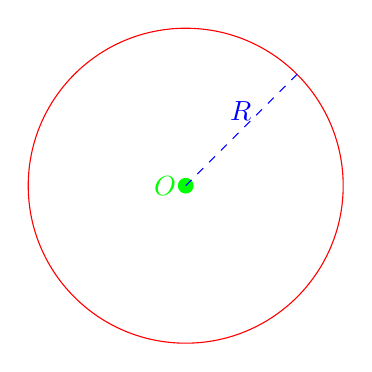
\begin{tikzpicture}
  \draw[red](0,0) circle(2);
  \path[fill=green][green] node[left]{$O$} circle(.1);
  \draw[dashed,blue](0,0) -- (.7,.7)node[above]{$R$} --
  (1.414213562373095,1.414213562373095);
\end{tikzpicture}
\end{center}

Note that when talking about formas planas, we can either consider only
the contour or also include the points in the interior ; with or without
specific terminology to make the distinction. In the previous example, we can
also consider the set of points that are at most at distance $R$ from $O$ and
call it the círculo ou disco.

Given two distinct
points $A$ and $B$ of the plane, we can consider the set of points
that are aligned with $A$ and $B$. This is called the uma reta and denoted
by $(AB)$. The point $A$ splits the reta $(AB)$ into two parts, called
semireta. The one containing $B$ is denoted ${\dot{A}B}$ or $[AB)$. The
subset of points between $A$ and $B$ is called um segmento (de reta) and
denoted by $[AB]$:

\begin{center}
\begin{tikzpicture}
  \draw[red](-5,0) -- (5,0) node[above]{$(AB)$};
  \path[fill=green][green] (0,0) node[above]{$A$} circle(.1);
  \path[fill=green][green] (2,0) node[above]{$B$} circle(.1);

  \begin{scope}[shift={(0,-2)}]
  \draw[dashed,blue](-5,0) -- (0,0);
  \draw[red](0,0) -- (5,0)  node[above]{${\dot{A}B} = [AB)$};
  \path[fill=green][green] (0,0) node[above]{$A$} circle(.1);
  \path[fill=green][green] (2,0) node[above]{$B$} circle(.1);
  \end{scope}

  \begin{scope}[shift={(0,-4)}]
  \draw[dashed,blue](-5,0) -- (0,0);
  \draw[dashed,blue](5,0) -- (0,0);
  \draw[red](0,0) -- (1,0)  node[above]{${[AB]}$} -- (2,0);
  \path[fill=green][green] (0,0) node[above]{$A$} circle(.1);
  \path[fill=green][green] (2,0) node[above]{$B$} circle(.1);
  \end{scope}
\end{tikzpicture}
\end{center}

Given pairwise distinct points $A_1, A_2, A_3, \ldots, A_n$ we can consider
the union of segmentos ${[A_1,A_2]}, {[A_2, A_3]}, {[A_3, A_4]},\ldots,
{[A_{n-1},A_n]}, {[A_{n},A_1]}$, which is called um polígono.
The points $A_1, A_2, \ldots$ are the vértices, while
the segmentos ${[A_1,A_2]}, {[A_2, A_3]}, {[A_3, A_4]},\ldots,$ are called the
lados.

\begin{center}
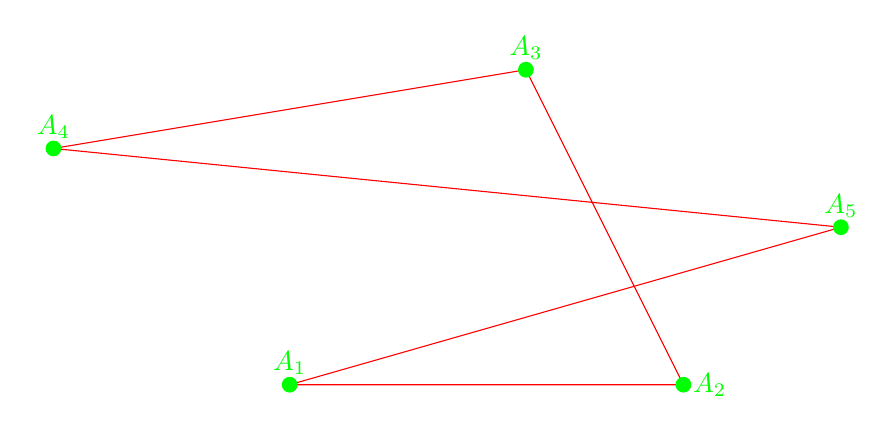
\begin{tikzpicture}
  \draw[red](0,0) -- (5,0) -- (3,4) -- (-3,3) -- (7,2) -- (0,0);

  \path[fill=green][green] (0,0) node[above]{$A_1$} circle(.1);
  \path[fill=green][green] (5,0) node[right]{$A_2$} circle(.1);
  \path[fill=green][green] (3,4) node[above]{$A_3$} circle(.1);
  \path[fill=green][green] (-3,3) node[above]{$A_4$} circle(.1);
  \path[fill=green][green] (7,2) node[above]{$A_5$} circle(.1);
\end{tikzpicture}
\end{center}

Um polígono is complexo if two non-consecutive lados intersect and otherwise
it is called simple. If we can find two points $P,Q$ belonging to um polígono
such that the segmento $[PQ]$ is not included in the interior of the polígono
then the polígono is côncavo ; otherwise it is convexo.

Um polígono can also be described from its lados.
Um polígono with $n$ lados is called
a $n$-gono with different terminology for various values of $n$:
triângulo (3 lados), quadrilátero (4 lados), pentágono (5 lados),
hexágono (6 lados), heptágono (7 lados), octógono (8 lados),
decágono (10 lados), dodecágono (12 lados) etc

If all angles are equal in measure and all sides have the same length then
the polígono is regulare.

\subsection*{Exercício 1}

Indique si los figuras siguientes son polígonos.

\begin{enumerate}

\item
 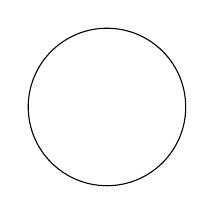
\begin{tikzpicture}
  \draw(0,0) circle(1);
 \end{tikzpicture}

\item
 \begin{tikzpicture}
   \draw (0,0) -- (1,0) -- (2,1) -- (1,2);
 \end{tikzpicture}

\item
  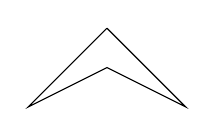
\begin{tikzpicture}
    \draw(1,1) --(0,0) -- (1,.5) -- (2,0) -- (1,1);
  \end{tikzpicture}

\item
 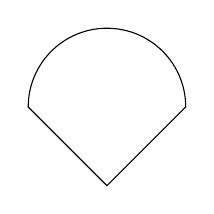
\begin{tikzpicture}
   \draw (0,0) -- (1,-1) -- (2,0) arc (0:180:1);
 \end{tikzpicture}

\item
  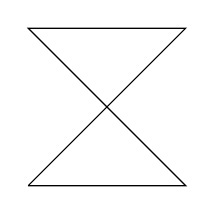
\begin{tikzpicture}
    \draw(0,0) --(2,0) -- (0,2) -- (2,2) -- (0,0);
  \end{tikzpicture}


\end{enumerate}

\subsection*{Exercício 2}

Sean $A,B,C,D,E,G,G,H,I$ los puntos de coordenadas
$(0,0)$, $(1,0)$, $(2,0)$,
$(0,1)$, $(1,1)$, $(2,1)$,
$(0,2)$, $(1,2)$ y $(2,2)$. Dibuja y describe los polígonos siguientes:

\begin{enumerate}
  \item $AHFBD$
  \item $DBFH$
  \item $ABIHE$
  \item $DBFG$
  \item $BCIH$
\end{enumerate}

\subsection*{Cuadriláteros}

Un cuadrilátero que tiene un par de lados paralelos es un trapezoide. Si
los lados opuestos son iguales y paralelos dos a dos, es llamado un
paralelogramo. Un paralelogramo con los cuatros lados paralelos es llamado
un rombo.

Un rectángulo tiene sus 4 ángulos de 90° y entonces es un
paralelogramo. Un cuadrado es un rectángulo con sus cuatro lados iguales y
por lo tanto es un cuadrilátero regular.

\subsection*{Exercício 3}

Dibuje:

\begin{enumerate}
\item un cuadrilátero simple convexo que no es un trapezoide.
\item un trapezoide que no es un paralelogramo.
\item un paralelogramo que es ni un rombo, ni un rectángulo.
\item un rombo que no es un cuadrado.
\item un rectángulo que no es un cuadrado.
\item un cuadrado.
\end{enumerate}

\subsection*{Formas espaciais}

Formas espaciais are sets of points in the three-dimensional space. For example,
given one point $O$ and a number $R > 0$ we can define the esfera
of center $O$ and radius $R$ as the set of points that are at distance $R$ from
$O$. Again, we can also consider points in the interior: the set of points
that are at most at distance $R$ are is called uma bola.

If we rotate a rectangle (including the interior) along one of its side,
we obtain a cylinder (including the interior). Similarly, if we rotate
a rectangle with one right angle along one its side side adjacent to that
right angle, we obtain a cone.

Just as we build um polígono simple from segmentos, we can build um poliedro from
polígonos. The polígonos are called faces and we keep the names vértices and
lados. We also keep the terminology côncavo and convexo. Um poliedro is regular
if all the faces are the same. Examples of well-known poliedros convexos are
tetraedro (made by four triangulares), cubo (made by six squares),
cuboid (made by six rectangles), parallelepiped (made by 6 parallelograms) or
pirâmide quadrangular (a quadrilateral basis and 4 triangles).
Um cubo or um tetraedro
made by equilateral (regular) triangles are examples of poliedros regulares.

\subsection*{Exercício 4}

Name the following formas espaciais.

\begin{enumerate}

\item
    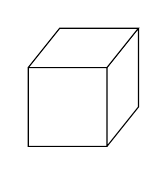
\begin{tikzpicture}
      \draw(0,0) -- (1,0) -- (1,1) -- (0,1) -- cycle
           (0,1) -- (.4,1.5) -- (1.4,1.5) -- (1,1)
           (1,0) -- (1.4,.5) -- (1.4,1.5);
    \end{tikzpicture}
    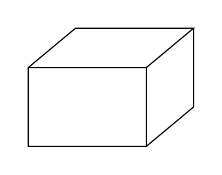
\begin{tikzpicture}[xscale=1.5]
      \draw(0,0) -- (1,0) -- (1,1) -- (0,1) -- cycle
           (0,1) -- (.4,1.5) -- (1.4,1.5) -- (1,1)
           (1,0) -- (1.4,.5) -- (1.4,1.5);
    \end{tikzpicture}
    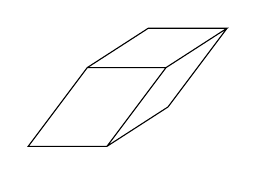
\begin{tikzpicture}[xslant=.75]
      \draw(0,0) -- (1,0) -- (1,1) -- (0,1) -- cycle
           (0,1) -- (.4,1.5) -- (1.4,1.5) -- (1,1)
      (1,0) -- (1.4,.5) -- (1.4,1.5);
   \end{tikzpicture}

\item 
  
\begin{tikzpicture}
    \begin{scope}[scale=2]
      \fill[red] (0,0) circle (0.5);
      \clip (0,0) circle (0.5);
      \shade[outer color=red, inner color=red!30] (-0.15,0.5) circle (0.7);
    \end{scope}
    \end{tikzpicture}
  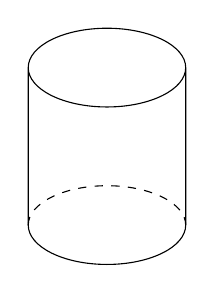
\begin{tikzpicture}
    \draw (0,0) ellipse(1 and .5)
          (-1,0) -- (-1,-2) arc(180:360:1 and .5) -- (1,0);
    \draw[dashed] (-1,-2) arc(180:0:1 and .5);
  \end{tikzpicture}
  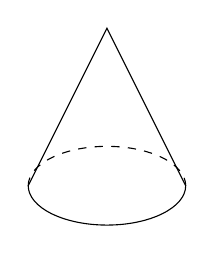
\begin{tikzpicture}
    \draw (0,0) -- (-1,-2) arc(180:360:1 and .5) -- cycle;
    \draw[dashed] (-1,-2) arc(180:0:1 and .5);
  \end{tikzpicture}

\item
    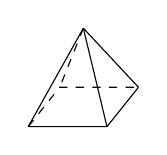
\begin{tikzpicture}
      \draw(0,0) -- (1,0) -- (1.4,.5);
      \draw (.7,1.25) -- (0,0);
      \draw (.7,1.25) -- (1,0);
      \draw (.7,1.25) -- (1.4,.5);
      \draw[dashed] (0,0) -- (.4,.5) -- (1.4,.5) (.7,1.25) -- (.4,.5);
    \end{tikzpicture}
    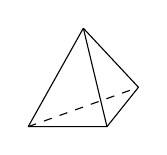
\begin{tikzpicture}
      \draw(0,0) -- (1,0) -- (1.4,.5);
      \draw (.7,1.25) -- (0,0);
      \draw (.7,1.25) -- (1,0);
      \draw (.7,1.25) -- (1.4,.5);
      \draw[dashed] (0,0) -- (1.4,.5);
    \end{tikzpicture}
      
\end{enumerate}

\subsection*{Planificação}

Um planificação uma forma espaciais é um arranjo de formas planas, que ao serem
dobrados retornam à forma espacial que lhe deu origem. As an example,
the following is um planificação of a cubo:

\begin{center}
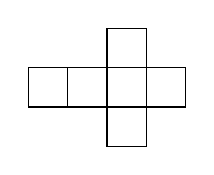
\begin{tikzpicture}
    \draw (0,0) -- (.5,0) -- (.5,.5) -- (0,.5) -- cycle
    (.5,0) -- (1,0) -- (1,.5) -- (.5,.5)
    (1,0) -- (1.5,0) -- (1.5,.5) -- (1,.5)
    (1.5,0) -- (2,0) -- (2,.5) -- (1.5,.5)
    (1,0) -- (1,-.5) -- (1.5,-.5) -- (1.5,0)
    (1,.5) -- (1,1) -- (1.5,1) -- (1.5,.5);
  \end{tikzpicture}
\end{center}

\subsection*{Exercício 5}

Identifica os sólidos geométricos planificados:

\begin{enumerate}
\item
  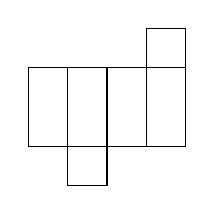
\begin{tikzpicture}
    \draw (0,0) -- (.5,0) -- (.5,1) -- (0,1) -- cycle
    (.5,0) -- (1,0) -- (1,1) -- (.5,1)
    (1,0) -- (1.5,0) -- (1.5,1) -- (1,1)
    (1.5,0) -- (2,0) -- (2,1) -- (1.5,1)
    (.5,0) -- (.5,-.5) -- (1,-.5) -- (1,0)
    (1.5,1) -- (1.5,1.5) -- (2,1.5) -- (2,1);
  \end{tikzpicture}

\item

  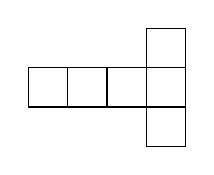
\begin{tikzpicture}
    \draw (0,0) -- (.5,0) -- (.5,.5) -- (0,.5) -- cycle
    (.5,0) -- (1,0) -- (1,.5) -- (.5,.5)
    (1,0) -- (1.5,0) -- (1.5,.5) -- (1,.5)
    (1.5,0) -- (2,0) -- (2,.5) -- (1.5,.5)
    (1.5,0) -- (1.5,-.5) -- (2,-.5) -- (2,0)
    (1.5,.5) -- (1.5,1) -- (2,1) -- (2,.5);
  \end{tikzpicture}

\item

  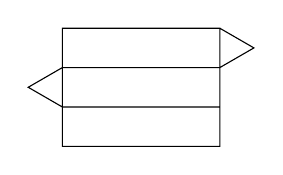
\begin{tikzpicture}
    \draw (0,0) -- (2,0) -- (2,.5) -- (0,.5) -- cycle
          (0,0) -- (0,-.5) -- (2,-.5) -- (2,0)
          (0,.5) -- (0,1) -- (2,1) -- (2,0.5)
          (0,0) -- (-0.4330127018922193,.25) -- (0,.5)
          (2,.5) -- (2.4330127018922193,.75) -- (2,1);
  \end{tikzpicture}

\item

  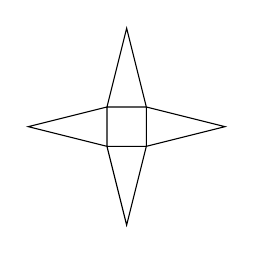
\begin{tikzpicture}
    \draw (0,0) -- (.5,0) -- (.5,.5) -- (0,.5) -- cycle
     (0,0) -- (-1,.25) -- (0,.5)
     (0,0) -- (.25,-1) -- (.5,0)
     (.5,0) -- (1.5,.25) -- (.5,.5)
     (0,.5) -- (.25,1.5) -- (.5,.5);
  \end{tikzpicture}

  
\end{enumerate}

\section{Perímetro e área}

The length of um segmento $[AB]$ is the distance between $A$ and $B$. We saw
in bimestre 2 that it was measured in meter or its múltiplos e submúltiplos da
unidade. The perímetro of um polígono is the sum of the length of its lados.
O tamanho da região interna do polígono se chama área.
Por exemplo, um retângulo de lados $5 \text{cm}$ e $7\text{cm}$ possui perímetro
$5+7+5+7=2{(5+7)} = 24\text{cm}$ e área $5 \times 7 = 35 \text{cm}^2$.

\begin{center}
 \begin{tikzpicture}
   \draw[color=red] (0,0) -- (2,0)node[below]{$7\text{cm}$} --
   (4,0) -- (4,1)node[right]{$5\text{cm}$} --
   (4,2) -- (2,2)node[above]{$7\text{cm}$} --
   (0,2) -- (0,1)node[left]{$5\text{cm}$} --
   (0,0);
 \end{tikzpicture}
\end{center}


\subsection*{Exercício 6}

\begin{enumerate}
\item
 Qual é o perímetro e a área de um quadrado de lado $3\text{cm}$?

\begin{center}
 \begin{tikzpicture}
   \draw[color=red] (0,0) --
   (2,0) -- (2,1)node[right]{$3\text{cm}$} --
   (2,2) --
   (0,2) --
   (0,0);
 \end{tikzpicture}
\end{center}

\item Seja $3\text{cm}$ e $4\text{cm}$ as longitudes das diagonais de um
  losango e $2.5\text{cm}$ a medida
  de um lado. Expresse o perímetro do losango e
  a área do losango (utilize a área do retângulo azul)?
  
\begin{center}
 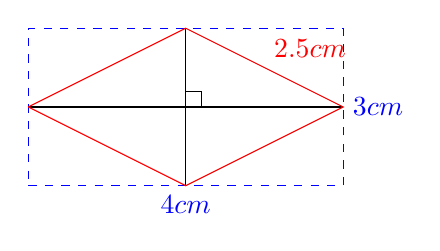
\begin{tikzpicture}
   \draw (2.2,0) -- (2.2,.2) -- (2,.2);
   \draw (0,0) -- (4,0);
   \draw (2,-1) -- (2,1);
   \draw[dashed,color=blue] (0,-1) --
   (2,-1)node[below]{$4\text{cm}$} --
   (4,-1) -- (4,0)node[right]{$3\text{cm}$} -- (4,1) -- (0,1) -- (0,-1);
   \draw[color=red] (0,0) -- (2,-1) -- (4,0) -- (3,.5)node[above right]{
   $2.5\text{cm}$} -- (2,1) -- (0,0);
 \end{tikzpicture}
\end{center}

\item Seja $5\text{cm}$ e $10\text{cm}$ as
  longitudes de um lado de um paralelogramo e $3\text{cm}$ a
  distância entre os dois lados paralelos de longitude $10\text{cm}$.
  Expresse o perímetro do paralelogramo e a área do paralelogramo.

\begin{center}
 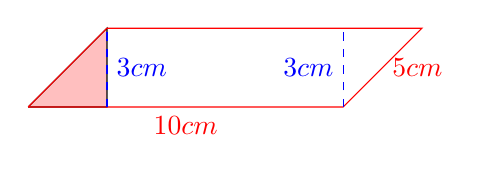
\begin{tikzpicture}
   \draw[color=transparent,fill=pink] (0,0) -- (1,0) -- (1,1) -- (0,0);
   \draw[color=red] (0,0) -- (2,0)node[below]{$10\text{cm}$} --
   (4,0) -- (4.5,.5)node[right]{$5\text{cm}$} -- (5,1) -- (1,1) -- (0,0);
   \draw[dashed,color=blue] (1,0) -- (1,.5)node[right]{$3\text{cm}$} -- (1,1);
   \draw[dashed,color=blue] (4,0) -- (4,.5)node[left]{$3\text{cm}$} -- (4,1);
 \end{tikzpicture}
\end{center}

\item Expresse o perímetro de um triângulo de lados $7\text{cm}$,
  $5\text{cm}$ e $6\text{cm}$.

\item Expresse a área de um triângulo de lado $8\text{cm}$ e altura $7\text{cm}$.
\begin{center}
 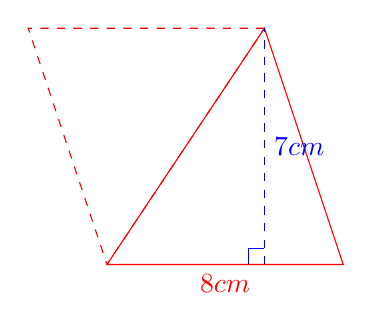
\begin{tikzpicture}
     \draw[color=red]
     (0,0) -- (1.5,0)node[below]{$8\text{cm}$} -- (3,0) -- (2,3) -- (0,0);
     \begin{scope}[rotate around={180:(1,1.5)}]
     \draw[color=red,dashed]
     (0,0) -- (3,0) -- (2,3) -- (0,0);
     \end{scope}
     \draw[color=blue,dashed](2,0)--(2,1.5)node[right]{$7\text{cm}$}--(2,3);
   \draw[color=blue](1.8,0)--(1.8,.2)--(2,.2);
 \end{tikzpicture}
\end{center}

\end{enumerate}

\subsection*{Exercício 7}

This grid is made of square of area $1 \text{m}^2$. Determine the area of
the following shapes:

\begin{center}
 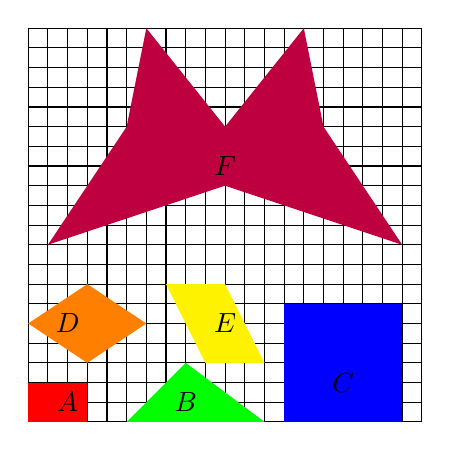
\begin{tikzpicture}[scale=.25]
   \draw (-10,-10) grid (10,10);

   \path[fill=red] (-10,-10) -- (-7,-10) -- (-7,-8) -- (-10,-8)
   (-8,-9) node{$A$};

   \path[fill=green] (-5,-10) -- (2,-10) -- (-2,-7) (-2,-9) node{$B$};

   \path[fill=blue] (3,-10) -- (9,-10) -- (9,-4) -- (3,-4)
   (6,-8)node{$C$};

   \path[fill=orange] (-10,-5) -- (-7,-7) -- (-4,-5) -- (-7,-3)
   (-8,-5)node{$D$};

   \path[fill=yellow] (-1,-7) -- (2,-7) -- (0,-3) -- (-3,-3)
   (0,-5) node{$E$};

   \path[fill=purple]
   (0,2) -- (0,5) -- (4,10) -- (5,5) -- (9,-1) -- cycle
   (0,2) -- (0,5) -- (-4,10) -- (-5,5) -- (-9,-1) -- cycle
   (0,3) node{$F$};
 \end{tikzpicture}
\end{center}

\section{Solução dos exercícios}

\subsection*{Exercício 1}

\begin{enumerate}

\item No (not made of a finite number of segments). This is a circle!
\item No (no cierra una región del plano).
\item Si (Polígono cóncavo)
\item No (tiene un segmento que no es recto)
\item Si (Polígono complejo)
\end{enumerate}

\subsection*{Exercício 2}

\begin{enumerate}
  \item Pentágono, complejo ($DB$ y $AH$ se intersectan).
  \item Cuadrilátero, simple, convexo, regular (cuadrado).
  \item Pentágono, simple, cóncavo.
  \item Pentágono, simple, convexo ($DB \neq GF$).
\end{enumerate}

\subsection*{Exercício 3}

\begin{enumerate}
\item
 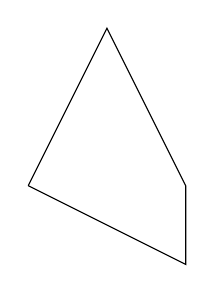
\begin{tikzpicture}
   \draw (0,0) -- (1,2) -- (2,0) -- (2,-1) -- (0,0);
 \end{tikzpicture}

\item
 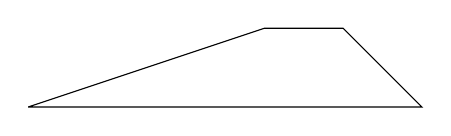
\begin{tikzpicture}
  \draw (0,0) -- (5,0) -- (4,1) -- (3,1) -- (0,0);
 \end{tikzpicture}
\item
 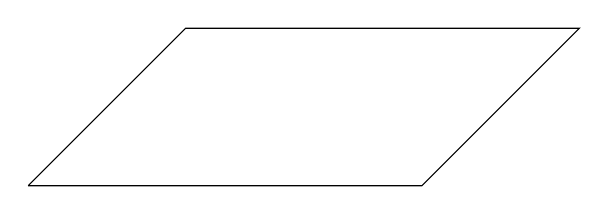
\begin{tikzpicture}
  \draw (0,0) -- (5,0) -- (7,2) -- (2,2) -- (0,0);
 \end{tikzpicture}
\item
 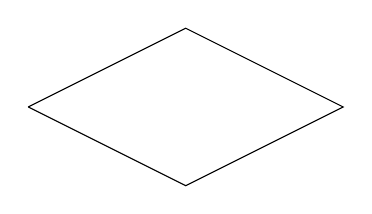
\begin{tikzpicture}
  \draw (0,0) -- (2,-1) -- (4,0) -- (2,1) -- (0,0);
 \end{tikzpicture}
\item
 \begin{tikzpicture}
  \draw (0,0) -- (4,0) -- (4,2) -- (0,2) -- (0,0);
 \end{tikzpicture}
\item
  Por ejemplo
 \begin{tikzpicture}
  \draw (0,0) -- (2,0) -- (2,2) -- (0,2) -- (0,0);
 \end{tikzpicture}, o con otra orientación:
 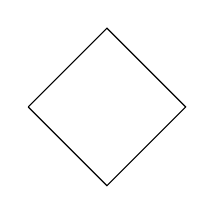
\begin{tikzpicture}
  \draw (0,0) -- (1,-1) -- (2,0) -- (1,1) -- (0,0);
 \end{tikzpicture}
\end{enumerate}

\subsection*{Exercício 4}

\begin{enumerate}
\item Cubo, cuboid, parallepiped
\item Esfera/Bola, cilindro, cone.
\item Pirâmide with square basis, tetraedro.
\end{enumerate}

\subsection*{Exercício 5}

Identifica os sólidos geométricos planificados:

\begin{enumerate}
\item cuboid
\item cubo
\item prisma com base um triangular equilateral
\item pirâmide with square basis
\end{enumerate}

\subsection*{Exercício 6}

\begin{enumerate}
\item $2 \times (3+3) = 12\text{cm}$, $3 \times 3 = 9\text{cm}^2$
\item $4 \times 2.5 = 10\text{cm}$, $\frac{3 \times 4}{2} = 6\text{cm}^2$
\item $2 \times {(10 + 5)} = 30\text{cm}$, $10 \times 3 = 30\text{cm}^2$
\item $7+5+6=18\text{cm}$
\item $\frac{7 \times 8}{2} = 28 \text{cm}^2$
\end{enumerate}

\subsection*{Exercício 7}

The first can easily be obtained using the formulas from the previous exercises
or by splitting each shape one into rectangles or halves of rectangles.
We get $A=6 \text{m}^2$, $B=10.5 \text{m}^2$, $C=36\text{m}^2$, $D=12\text{m}^2$,
$E=12\text{m}^2$.

The last one has an obvious symmetry along the $y$-axis. We can obtain the area
of each half as follows:
  
\begin{center}
 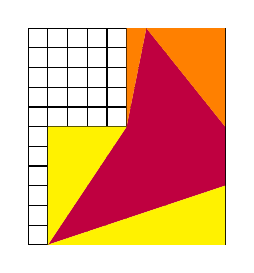
\begin{tikzpicture}[scale=.25]
   \draw (-10,-1) grid (0,10);
   \path[fill=purple] (0,2) -- (0,5) -- (-4,10) -- (-5,5) -- (-9,-1) -- cycle;
   \path[fill=orange] (0,5) -- (0,10) -- (-4,10) -- cycle;
   \path[fill=orange] (-4,10) -- (-5,10) -- (-5,5) -- cycle;
   \path[fill=yellow] (-5,5) -- (-9,5) -- (-9,-1) -- cycle;
   \path[fill=yellow] (-9,-1) -- (0,-1) -- (0,2) -- cycle;
 \end{tikzpicture}
\end{center}
The area in yellow is $12 + 13.5 = 25.5\text{m}^2$, the area
in orange is $2.5 + 10 = 12.5 \text{m}^2$. Finally the area in purple is
$2 \times {(25 + 54 - 25.5 - 12.5)} = 82 \text{m}^2$.
